% uw-wkrpt-ece.tex - An example work report that uses uw-wkrpt.cls
% Copyright (C) 2002,2003  Simon Law
% 
% This program is free software; you can redistribute it and/or modify
% it under the terms of the GNU General Public License as published by
% the Free Software Foundation; either version 2 of the License, or
% (at your option) any later version.
% 
% This program is distributed in the hope that it will be useful,
% but WITHOUT ANY WARRANTY; without even the implied warranty of
% MERCHANTABILITY or FITNESS FOR A PARTICULAR PURPOSE.  See the
% GNU General Public License for more details.
% 
% You should have received a copy of the GNU General Public License
% along with this program; if not, write to the Free Software
% Foundation, Inc., 59 Temple Place, Suite 330, Boston, MA  02111-1307  USA
%
%%%%%%%%%%%%%%%%%%%%%%%%%%%%%%%%%%%%%%%%%%%%%%%%%%%%%%%%%%%%%%%%%%%%%
%
% We begin by calling the workreport class which includes all the
% definitions for the macros we will use.
\documentclass[ece]{uw-wkrpt}
\usepackage[left=1.5in,top=1.0in,right=1.0in]{geometry}
\usepackage{verbatim}
\usepackage{moreverb}


% We will use some packages to add functionality
\usepackage{graphicx} % Include graphic importing

% Now we will begin writing the document.
\begin{document}

%%%%%%%%%%%%%%%%%%%%%%%%%%%%%%%%%%%%%%%%%%%%%%%%%%%%%%%%%%%%%%%%%%%%%
%% IMPORTANT INFORMATION
%%%%%%%%%%%%%%%%%%%%%%%%%%%%%%%%%%%%%%%%%%%%%%%%%%%%%%%%%%%%%%%%%%%%%

%% First we, should create a title page.  This is done below:
% Fill in the title of your report.
\title{ ECE 457B: Facereader }



\author{Kiril Gorovoy}
% Fill in your student ID number.
\uwid{}

% Fill in your home address.
\address{256 Phillip St. Unit 45.,\\*
         Waterloo, ON\ \ N2L 6B6}

% Fill in your employer's name.
\employer{ dd }

% Fill in your employer's city and province.
\employeraddress{Summit, NJ}

% Fill in your school's name.
\school{University of Waterloo}

% Fill in your faculty name.
\faculty{Faculty of Engineering}

% Fill in your e-mail address.
\email{ja2green@engmail.uwaterloo.ca}

% Fill in your term.
\term{4B}

% Fill in your program.
\program{Computer Engineering}



% If you are writing a "Confidential 1" report, uncomment the next line.
%\confidential{Confidential-1}

% If you want to specify the date, fill it in here.  If you comment out
% this line, today's date will be substituted.

% Now, we ask LaTeX to generate the title.
\maketitle

%%%%%%%%%%%%%%%%%%%%%%%%%%%%%%%%%%%%%%%%%%%%%%%%%%%%%%%%%%%%%%%%%%%%%
%% FRONT MATTER
%%%%%%%%%%%%%%%%%%%%%%%%%%%%%%%%%%%%%%%%%%%%%%%%%%%%%%%%%%%%%%%%%%%%%
%% \frontmatter will make the \section commands ignore their numbering,
%% it will also use roman page numbers.
\frontmatter

\tableofcontents
\listoffigures
\listoftables

%%%%%%%%%%%%%%%%%%%%%%%%%%%%%%%%%%%%%%%%%%%%%%%%%%%%%%%%%%%%%%%%%%%%%
%% REPORT BODY
%%%%%%%%%%%%%%%%%%%%%%%%%%%%%%%%%%%%%%%%%%%%%%%%%%%%%%%%%%%%%%%%%%%%%
%% \main will make the \section commands numbered again,
%% it will also use arabic page numbers.
\mainmatter

\section{Introduction}
This report analyzes the suitability of three different neural network learning algorithms in the context of recognizing emotions from images of human facial expressions. 
Using an analytical approach, conclusions will be drawn concerning which network type provides the best solution to this problem. Also, there will be inquiry into why each neural network is able (or not able) to  adequately perform the learning task. 

\subsection{Problem}
A selection of neural networks should be trained to detect human emotion from a 640x480 facial image. The emotions that need to be detected are: sad, smiling, calm and astonished.  A subset of the pixels in this image should be extracted manually and used as inputs to each neural network. The global data set should consist of sixteen people (mix of male and female) displaying each of the four emotions. 

\subsection{Methodology}
We chose to analyze a simple feedforward network trained using backpropogation, a radial basis network and  a self organizing map. An analysis of these network types should provide insight into the feasibility of supervised vs unsupervised learning methods for this problem. In order to effectively discern emotion from the facial images, the pixels around the mouth area were used. The highest variation in the emotions we are concerned with occurs in this region of the image. The pixels extracted from this area were used as inputs to our neural networks. 

\subsection{Background}
This section will provide a brief high level overview of the neural network types included in the analysis.
\subsubsection{ Feedforward with Backpropogation}
blah
\subsubsection{Radial Basis Networks}
blah
\subsubsection{Self Organizing Maps} 
blah




\pagebreak

\section{Implementation}
Each neural network was implemented using Matlab and the Matlab Neural Network Toolbox (NNT). NNT provides matlab functions for designing, implementing, visualizing and simulating different types of neural networks [1]. The three types of networks we chose for analysis are supported under the NNT, which greatly simplified the process and allowed us to focus on optimization rather than unimportant implementation details.

\subsection{Dataset}
As per the requirements, we gathered images of sixteen people displaying each emotion for our global dataset, eight males and eight females. Each picture was taken using a low quality webcam of 640x480 resolution, in a variety of lighting conditions.

\begin{figure}
	\centering
		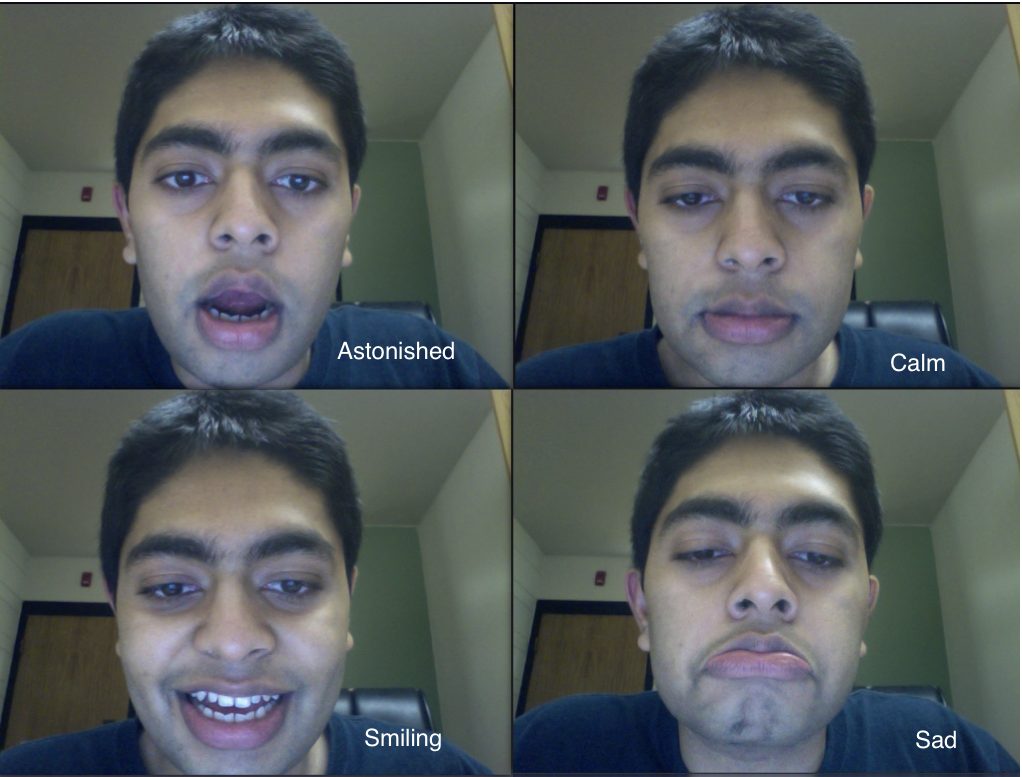
\includegraphics[scale=0.3]{sample.png}
	\caption{Example set of input facial images}
	\label{fig:binding}
\end{figure}


\subsection{Feature Extraction}
A subset of  the facial image pixels must be selected to generate inputs for the networks. The project specifications require that 400 pixels from each image be used as input nodes. To satisfy this requirement, a rectangular subset of the facial image is selected manually by the user, and this region is subsequently scaled to a 24x16 area.
\\
 Additionally, in order to extract the most relevant input data for our networks, several different feature extraction methods were experimented with. These include:
 
 \begin{itemize}
\item \textbf{Grey Scaling}

\item \textbf{Red Component}
\item \textbf{ Normalized Grey Scale}
\item \textbf{Normalized Red Component}
\end{itemize}
 



\subsection{Testing Methodology}




\subsection{User Interface}
The UI was also implemented using Matlab. It allows the user to select an area of the image for feature extraction and a network type for testing. Based on these inputs parameters, the user can then test the network and the identified emotion will be output to the user.  The networks have already been pre trained and cached, so the response should appear immediately. 

{screenshot of UI}

\pagebreak

\section{Supervised Learning Using Backpropogation}
\subsection{ Algorithm}
\subsection{Results}
\begin{table}
\begin{center}
    \begin{tabular}{ | l | l | l | l | l | l |}
    \hline
    Solution & Re-use &Testing & Performance & Cost & Total  \\ \hline
    Traditional Code Behind & 0 & 0 & 0 & 1 &  \textbf 1  \\ \hline
    MVP & 1 & 1 & 0 & 0 &  \textbf 2  \\ \hline
    MVVM & 2 & 2 & 1 & 0 &  \textbf 5  \\ \hline
    \hline
    \end{tabular}
\end{center}
\caption{ Overall Scores}
	\label{table:overall}
\end{table}

\section {Radial Basis Network}
\subsection{ Algorithm}
\subsection{Results}
\begin{table}
\begin{center}
    \begin{tabular}{ | l | l | l | l | l | l |}
    \hline
    Solution & Re-use &Testing & Performance & Cost & Total  \\ \hline
    Traditional Code Behind & 0 & 0 & 0 & 1 &  \textbf 1  \\ \hline
    MVP & 1 & 1 & 0 & 0 &  \textbf 2  \\ \hline
    MVVM & 2 & 2 & 1 & 0 &  \textbf 5  \\ \hline
    \hline
    \end{tabular}
\end{center}
\caption{ Overall Scores}
	\label{table:overall}
\end{table}
                                                                                                                                                                                                                                                                                                                                                                                                                                                                                                                                                                                                                                                                                                                                                                                                                                                                                                                                                                                                                                                                                                                                                                                                                                                                                                                                                                                                                                                                                                                                                                                                                                                                                                                                                                                                                                                                                                                                                                                                                                                                                                                                                                                                                                                                                                                                                                                                                                                                                                                                                                                                                                                                                                                                                                                                                                                                                                                                                                                                                                                                                                                                                                                                                                                                                                                                                                                                                                                                                                                                                                                                                                                                                                                                                                                                                                                                                                                                                                                                                                                                                                                                                                                                                                                                                                                                                                                                                                                                                                                                                                                                                                                                                                                                                                                                                                                                                                                                                                                                                                                                                                                                                                                                                                                                                                                                                                                                                                                                                                                                                                                                                                                                                                                                                                                                                                                                                                                                                                                                                                                                                                                                                                                                                                                                                                                                                                                                                       
\section{ Unsupervised Learning Based on Kohonen Learning Rate    }
\subsection{ Algorithm}
\subsection{Results}
\begin{table}
\begin{center}
    \begin{tabular}{ | l | l | l | l | l | l |}
    \hline
    Solution & Re-use &Testing & Performance & Cost & Total  \\ \hline
    Traditional Code Behind & 0 & 0 & 0 & 1 &  \textbf 1  \\ \hline
    MVP & 1 & 1 & 0 & 0 &  \textbf 2  \\ \hline
    MVVM & 2 & 2 & 1 & 0 &  \textbf 5  \\ \hline
    \hline
    \end{tabular}
\end{center}
\caption{ Overall Scores}
	\label{table:overall}
\end{table}
 
\section{Conclusion}





%%%%%%%%%%%%%%%%%%%%%%%%%%%%%%%%%%%%%%%%%%%%%%%%%%%%%%%%%%%%%%%%%%%%%
%% BACK MATTER
%%%%%%%%%%%%%%%%%%%%%%%%%%%%%%%%%%%%%%%%%%%%%%%%%%%%%%%%%%%%%%%%%%%%%
%% \backmatter will make the \section commands ignore their numbering,
\backmatter


% Here, we insert a References section, which will be formatted properly.
% The list of works you have referenced should be in FILENAME.bib,
% which will be workreport-sample.bib, if you use the command below.
%
% Note, you will need to process the document in a certain order.  First,
% run LaTeX.  The % first pass will allow LaTeX to build a list of 
% references, it may % emit warning messages such as:
%   LaTeX Warning: Reference `app:gnugpl' on page 4 undefined on input line 277.
%   LaTeX Warning: There were undefined references.
% This is normal.  Now you run BiBTeX in order to generate the proper
% layout for the references.  After this, you run LaTeX once more.
\bibliography{uw-wkrpt-bib}

%%%%%%%%%%%%%%%%%%%%%%%%%%%%%%%%%%%%%%%%%%%%%%%%%%%%%%%%%%%%%%%%%%%%%
%% APPENDICES
%%%%%%%%%%%%%%%%%%%%%%%%%%%%%%%%%%%%%%%%%%%%%%%%%%%%%%%%%%%%%%%%%%%%%
%% \appendix will reset \section numbers and turn them into letters.
%%
%% Don't forget to refer to all your appendices in the main report.

\end{document}
